\subsection{Offline inference and hardware acceleration}

The implementation reuses Ultralytics pose estimation~\cite{ultralyticsPose}, the Hailo inference runtime, and Mamba state-space operators~\cite{gu2023mamba}; TCNTE~\cite{yu2025tcnte} provides a comparison baseline. The classifier combines bidirectional temporal processing, attention, masking, and pose-quality pooling. FallGuard integrates it with local alert storage, deferred cloud synchronization, and a monitoring interface.

The project repository provides model and metric code, experiment configurations, manuscript sources, and aggregate results. The separate deployment archive contains the edge runtime and cloud synchronization services; credentials and runtime databases are excluded. Training runs retain resolved configurations and environment metadata. Original training manifests and pose caches are absent from the available materials. Rebuilding the pipeline therefore requires reconstructing these inputs before an exact replay of the archived training runs is possible.

The edge runtime reads a USB camera or a local video. FFmpeg decodes AV1 inputs and preserves their presentation timestamps. YOLOv8s-pose on Hailo produces 17 COCO keypoints and a person confidence. HailoRT converts the network outputs to floating-point tensors before bounding-box and keypoint decoding. The highest-confidence person supplies the 12 body joints used by the temporal model. A CPU ONNX pose backend supports operation without the accelerator.

A timestamped buffer forms one-second windows up to five times per second. Each window is interpolated to 30 samples and normalized as in training. The three quality features of Eq.~\eqref{eq:quality_features} form the quality input. ONNX Runtime executes MaskedBiMamba locally on the Pi CPU. Camera acquisition runs in a separate thread so that a slow inference call does not accumulate old images.

\subsection{Record storage and synchronization}

SQLite commits each prediction together with its updated alert state. A separate outbox service exposes pending records through the private network. The cloud importer deduplicates records by identifier and retains the original observation time. The sender marks records as delivered only after the cloud confirms its database transaction. Polling resumes automatically after connectivity returns, with pending batches drained before returning to the normal polling interval.

\subsection{Detection interface}

Figure~\ref{fig:dashboard} shows the monitoring interface. The operator selects an input source, views the pose and fall probability, and reviews the current alert state. Event history supports acknowledgement with notes. Camera start and stop controls are available for the Pi input. A separate local page displays annotated camera frames, current classification, and pending-record counts directly on the Pi during network outages. Local integration tests cover alert transitions, record persistence across restarts, retry handling, and acknowledgement.

\begin{figure}[tbp]
    \centering
    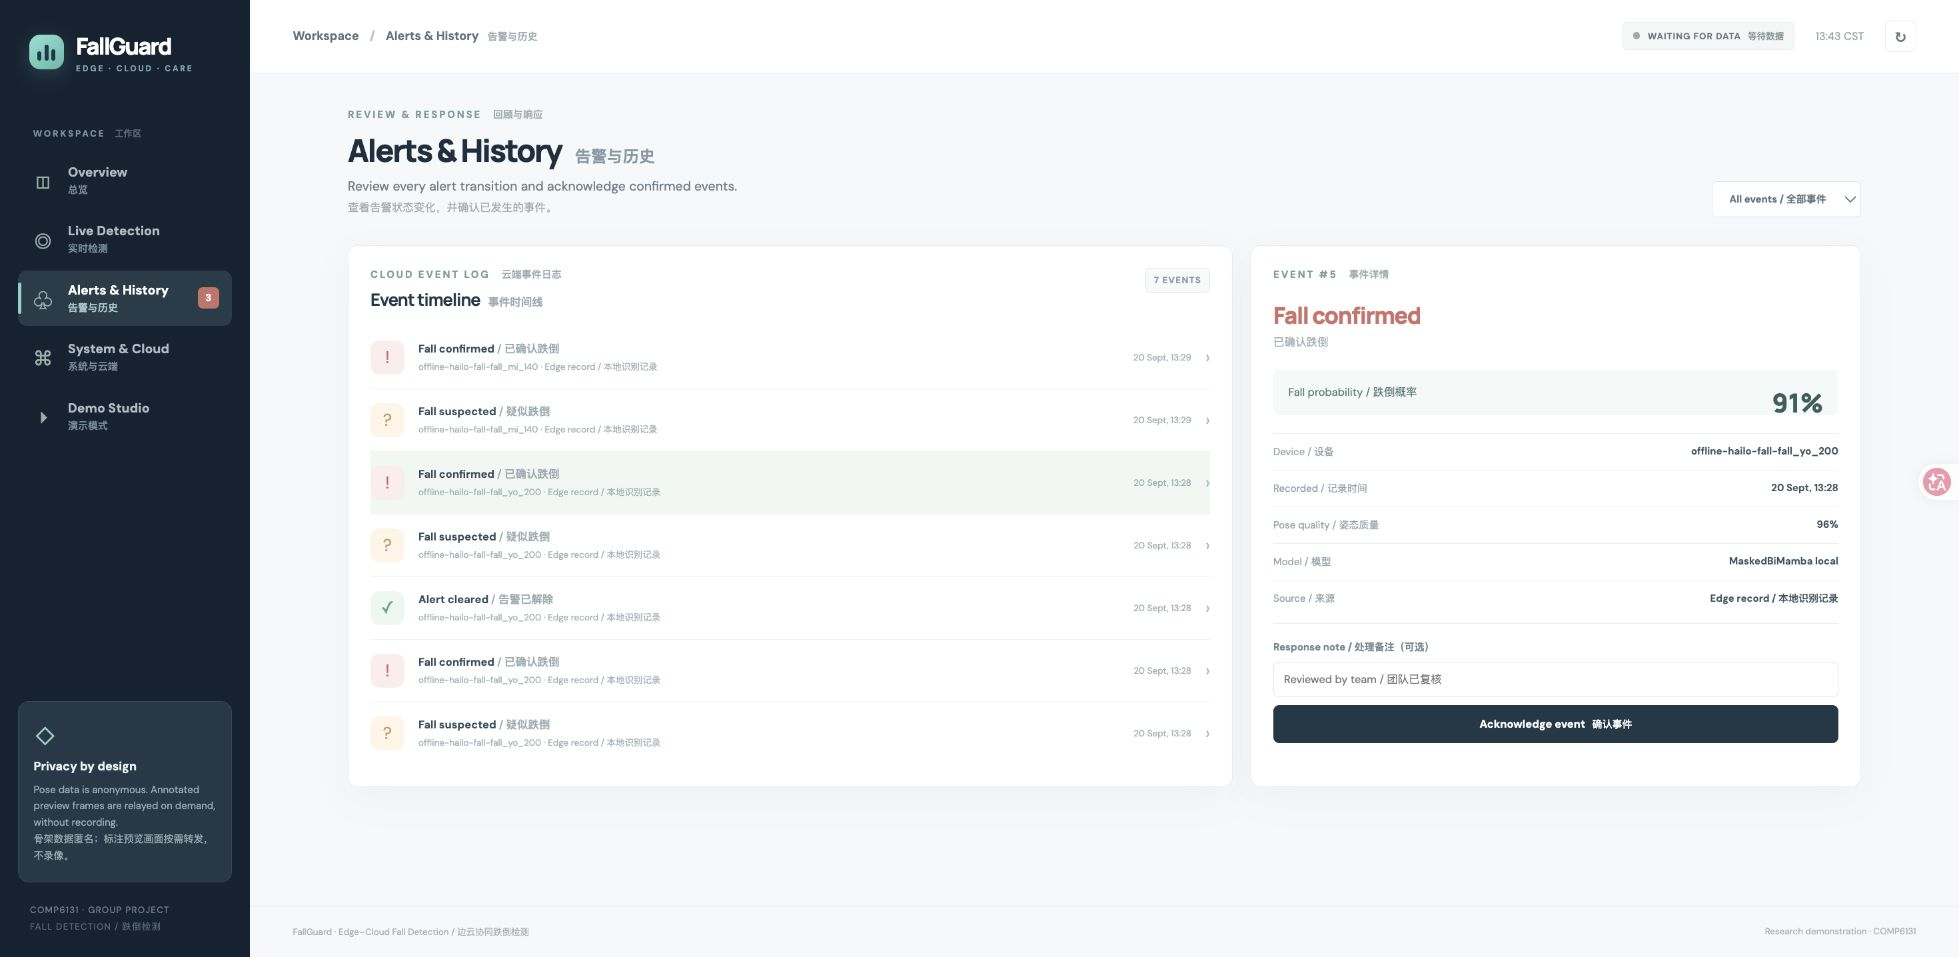
\includegraphics[width=\columnwidth]{figs/detection_system_edge_records.png}
    \caption{FallGuard event interface displaying actual Raspberry Pi predictions on OmniFall-Synthetic videos. The local review instance shows the event timeline, model score, original recording time, and acknowledgement controls.}
    \label{fig:dashboard}
\end{figure}
